%!TEX root = syntheyes15.tex

\section{Synthetic data generation}

\cite{MIL-STD-1472G} -- cite for range of eye rotation.

\begin{figure}
    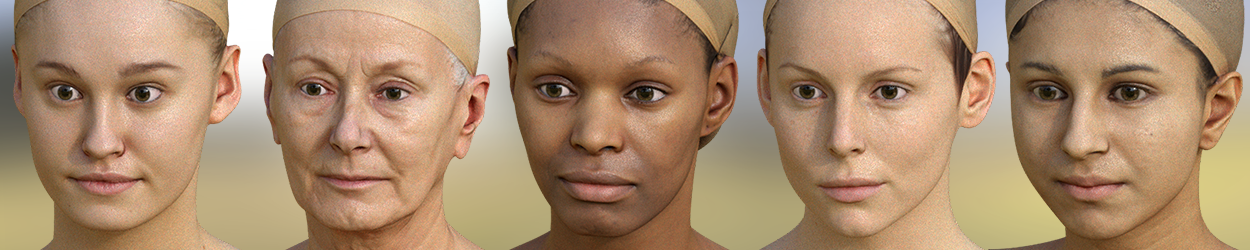
\includegraphics[width=\columnwidth]{participants_f} \par \smallskip
    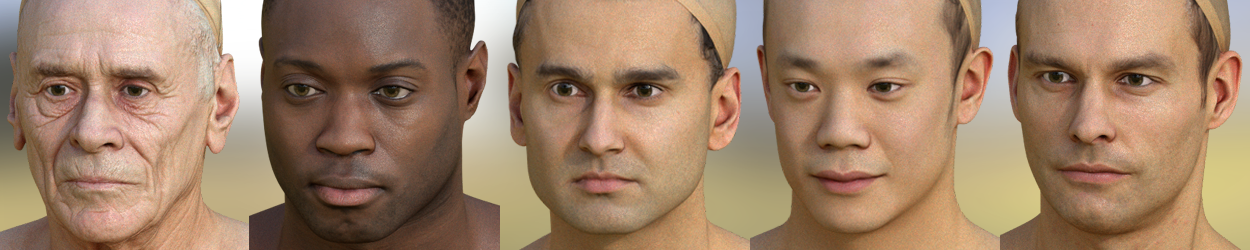
\includegraphics[width=\columnwidth]{participants_m}
    \caption{Our suite of female and male head models for rendering.}
    \label{fig:participants}
\end{figure}

\begin{figure}
    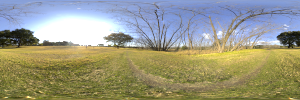
\includegraphics[width=0.24\columnwidth]{env1} \hfill
    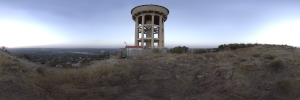
\includegraphics[width=0.24\columnwidth]{env2} \hfill
    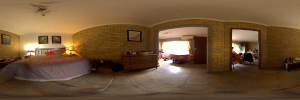
\includegraphics[width=0.24\columnwidth]{env3} \hfill
    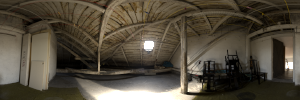
\includegraphics[width=0.24\columnwidth]{env4} \par \vspace{-0.01em}
    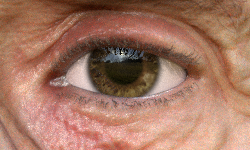
\includegraphics[width=0.24\columnwidth]{male01_env1} \hfill
    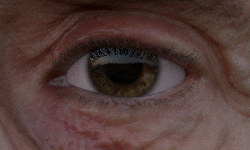
\includegraphics[width=0.24\columnwidth]{male01_env2} \hfill
    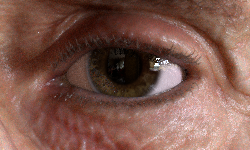
\includegraphics[width=0.24\columnwidth]{male01_env3} \hfill
    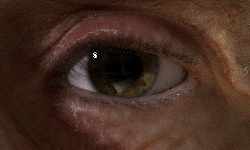
\includegraphics[width=0.24\columnwidth]{male01_env4}
    \caption{Different environments.}
    \label{fig:participants}
\end{figure}